% !TEX root = ../../../main.tex
% 来源：中学数学实验教材·第三册（高中数学）
% 章节：不等式和解不等式 / 大小次序与不等式
% 原始文件：3.tex，行 100-112
% 类型：tikz
% ---
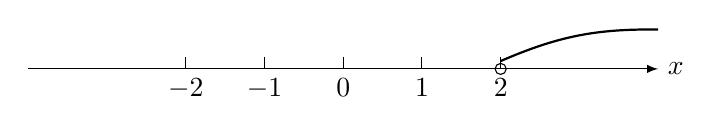
\begin{tikzpicture}[>=latex]
    \draw[->] (-4,0)--(4,0)node [right]{$x$};

\foreach \x in {-2,-1,...,2}
{
    \draw (\x,.15)--(\x, 0)node[below]{$\x$};
}
\draw (2,0) circle (2pt);

\draw[thick]  (2,0.1) to [bend left=12] (4,.5);


\end{tikzpicture}
